\documentclass[11pt,a4paper]{article}

\usepackage[margin=2.2cm]{geometry}
\usepackage[T1]{fontenc}
\usepackage{lmodern}
\usepackage{microtype}
\usepackage{graphicx}
\usepackage{booktabs}
\usepackage{tabularx}
\usepackage{amsmath}
\usepackage{xcolor}
\usepackage{float}
\usepackage{caption}
\usepackage{subcaption}
\usepackage{enumitem}
\usepackage{fancyhdr}
\usepackage{tikz}
\usetikzlibrary{arrows.meta,positioning,fit,calc}
\usepackage[hidelinks]{hyperref}

\definecolor{accent}{HTML}{0B6A87}
\definecolor{ink}{HTML}{15181C}
\definecolor{muted}{HTML}{687079}
\definecolor{panel}{HTML}{EEF2F5}

\graphicspath{{figures/}}
\captionsetup{font=small,labelfont=bf,margin=0.5cm}
\setlist{itemsep=2pt,topsep=4pt}
\setlength{\parskip}{4pt}
\pagestyle{fancy}
\fancyhf{}
\fancyhead[L]{\small\color{muted}CareLoop-Edge: project report}
\fancyhead[R]{\small\color{muted}\thepage}
\renewcommand{\headrulewidth}{0.3pt}

% a screenshot: full width, never taller than most of the page
\newcommand{\shot}[3][0.82]{%
  \begin{figure}[H]\centering
  \includegraphics[width=\linewidth,height=#1\textheight,keepaspectratio]{#2}
  \caption{#3}\label{fig:#2}\end{figure}}

\tikzset{
  box/.style={draw=accent!70, fill=panel, rounded corners=1.5pt, align=center, font=\small, inner sep=5pt, text width=#1},
  box/.default=3.2cm,
  arr/.style={-{Stealth[length=2.2mm]}, thick, color=ink!70},
  lab/.style={font=\scriptsize\itshape, color=muted, align=center}
}

\begin{document}

% ------------------------------------------------------------------------------------------------ title
\begin{titlepage}
\centering
\vspace*{2.5cm}
{\color{accent}\rule{\linewidth}{1.2pt}}\\[14pt]
{\Huge\bfseries CareLoop-Edge}\\[8pt]
{\Large Assistive AI follow-up and continuity of care for brain MRI\\ on a Raspberry Pi}\\[10pt]
{\color{accent}\rule{\linewidth}{1.2pt}}\\[30pt]
{\large Project report}\\[60pt]
\begin{tabular}{rl}
\textbf{Author} & Tanmay Rawal \\
\textbf{Repository} & \url{https://github.com/TanmayRawal/CareloopEdge} \\
\textbf{Release described} & model \texttt{mri/0.3.0}, portal commit \texttt{2c90ba2} \\
\textbf{Date} & October 2026 \\
\end{tabular}
\vfill
{\small\color{muted} Research prototype on public data. It is not a medical device and is not intended for clinical decisions.
Every AI result in the system is reviewed and signed by a radiologist before a patient sees anything.}
\end{titlepage}

\begin{abstract}
\noindent CareLoop-Edge is a brain-MRI decision-support and follow-up system that runs entirely on a Raspberry Pi in a
clinic. A patient, or a health worker on their behalf, uploads a single image or a whole MRI study. A quantised
ResNet-50 classifier with a segmentation head analyses it on the device. The result goes to a radiologist's worklist
with calibrated probabilities, a 95\% prediction set, an exact lesion-focused Grad-CAM explanation and the lesion
outline. The radiologist signs the report and chooses the next step (consultation, repeat MRI or referral). The
care-loop part of the system then makes sure that step happens: appointment booking, reminders, a risk-ranked
follow-up worklist for the coordinator, referral tracking and analytics on loop closure.

The model is trained on a PC, audited for data leakage, quantised to INT8, and reaches the device as a signed and
encrypted bundle from a self-hosted registry. Patient data is encrypted at rest and every access is written to a
tamper-evident audit log. After feedback from a radiologist that diagnosis is made from the whole study, the model was
evaluated on complete 3D patient scans, retrained, and released as \texttt{mri/0.3.0}. On held-out patients it
reaches a tumour-type macro-F1 of 0.98, a slice-level tumour AUROC of 0.95 and a 5\% false-alarm rate on healthy
volunteers, meeting all three pre-registered targets.
\end{abstract}

\tableofcontents
\newpage

% ================================================================================================ 1
\section{Problem and goals}
In district hospitals and screening camps a brain MRI may be acquired, read once, and then the patient is lost. The
nearest neurosurgeon or neuroradiologist can be 60--100\,km away, and nobody tracks whether the follow-up scan, the
consultation or the referral ever happened. The project addresses two linked problems:
\begin{enumerate}
\item \textbf{Reading support at the edge.} Give the radiologist a fast, explainable second look at the study,
computed on a low-cost device in the clinic, with no cloud GPU and no patient data leaving the site.
\item \textbf{Closing the care loop.} After the report is signed, track the patient until the next step chosen by the
radiologist has actually happened, and make the patients at risk of being lost visible to the care team.
\end{enumerate}
Design principles that run through the whole system: the AI assists and the doctor decides; patients never see raw
AI output; every number shown is measured, not estimated; and the system keeps working offline.

% ================================================================================================ 2
\section{Project workflow}
Figure~\ref{fig:workflow} summarises the order in which the work was done. Each stage produced a measured result
recorded in \texttt{docs/FINDINGS.md}; several stages changed the plan of the next one.

\begin{figure}[H]\centering
\resizebox{\linewidth}{!}{%
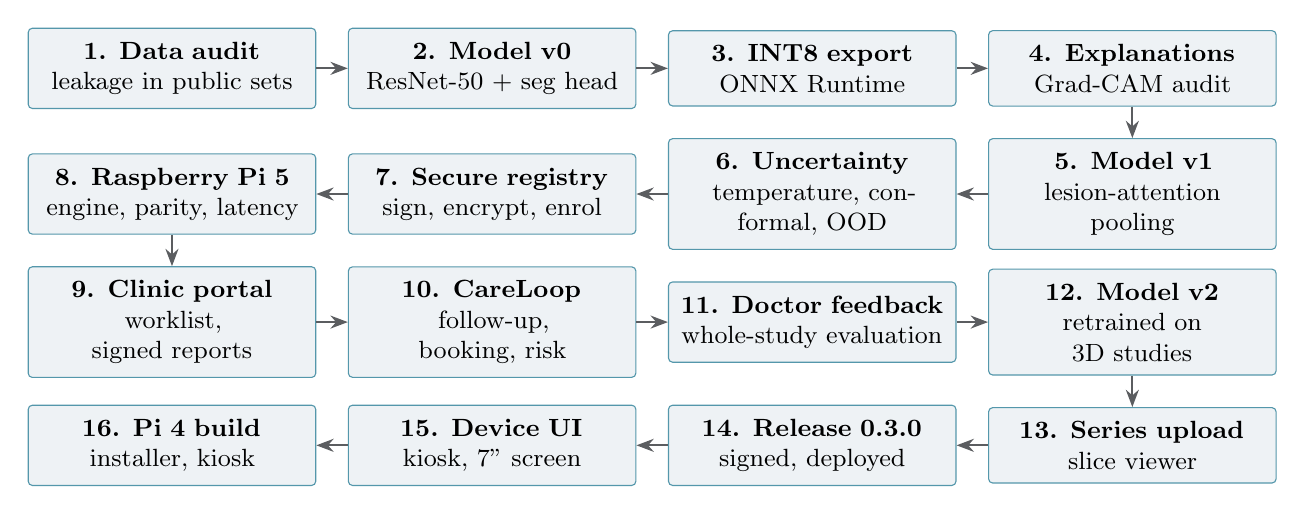
\begin{tikzpicture}[node distance=4mm and 4mm]
\node[box=3.3cm] (a) {\textbf{1. Data audit}\\ leakage in public sets};
\node[box=3.3cm, right=of a] (b) {\textbf{2. Model v0}\\ ResNet-50 + seg head};
\node[box=3.3cm, right=of b] (c) {\textbf{3. INT8 export}\\ ONNX Runtime};
\node[box=3.3cm, right=of c] (d) {\textbf{4. Explanations}\\ Grad-CAM audit};
\node[box=3.3cm, below=of d] (e) {\textbf{5. Model v1}\\ lesion-attention pooling};
\node[box=3.3cm, left=of e] (f) {\textbf{6. Uncertainty}\\ temperature, conformal, OOD};
\node[box=3.3cm, left=of f] (g) {\textbf{7. Secure registry}\\ sign, encrypt, enrol};
\node[box=3.3cm, left=of g] (h) {\textbf{8. Raspberry Pi 5}\\ engine, parity, latency};
\node[box=3.3cm, below=of h] (i) {\textbf{9. Clinic portal}\\ worklist, signed reports};
\node[box=3.3cm, right=of i] (j) {\textbf{10. CareLoop}\\ follow-up, booking, risk};
\node[box=3.3cm, right=of j] (k) {\textbf{11. Doctor feedback}\\ whole-study evaluation};
\node[box=3.3cm, right=of k] (l) {\textbf{12. Model v2}\\ retrained on 3D studies};
\node[box=3.3cm, below=of l] (m) {\textbf{13. Series upload}\\ slice viewer};
\node[box=3.3cm, left=of m] (n) {\textbf{14. Release 0.3.0}\\ signed, deployed};
\node[box=3.3cm, left=of n] (o) {\textbf{15. Device UI}\\ kiosk, 7" screen};
\node[box=3.3cm, left=of o] (p) {\textbf{16. Pi 4 build}\\ installer, kiosk};
\draw[arr] (a)--(b); \draw[arr] (b)--(c); \draw[arr] (c)--(d); \draw[arr] (d)--(e); \draw[arr] (e)--(f);
\draw[arr] (f)--(g); \draw[arr] (g)--(h); \draw[arr] (h)--(i); \draw[arr] (i)--(j); \draw[arr] (j)--(k);
\draw[arr] (k)--(l); \draw[arr] (l)--(m); \draw[arr] (m)--(n); \draw[arr] (n)--(o); \draw[arr] (o)--(p);
\end{tikzpicture}}
\caption{Order of the work. Stages 1--8 build and secure the model; 9--10 build the clinical product; 11--14 respond to
a radiologist's feedback that diagnosis is made from the whole study; 15--16 turn it into a stand-alone device.}
\label{fig:workflow}
\end{figure}

\begin{enumerate}[label=\textbf{\arabic*.}]
\item \textbf{Data audit.} Public brain-tumour MRI benchmarks were found to leak heavily: 566 of the 1{,}000 official
BRISC test images are copies (462 mirrored) of training images, and other public sets largely duplicate BRISC. A
flip-aware similarity search defines leakage-free, patient-grouped splits used for every result in this report.
\item \textbf{Model v0.} A ResNet-50 classifier (glioma, meningioma, pituitary tumour, no tumour) with an FPN
segmentation head, trained on the leakage-free split.
\item \textbf{INT8 export.} ONNX export and static INT8 quantisation (96.6\,MB to 24.7\,MB). The audit showed that
v0 INT8 silently lost 11 macro-F1 points on external data; external INT8 evaluation became part of acceptance.
\item \textbf{Explanations.} Grad-CAM, LayerCAM, Finer-CAM and ShapleyCAM were evaluated against expert tumour masks.
The v0 maps put only 15\% of their evidence inside the tumour, and pituitary maps highlighted anatomy, not tumour.
\item \textbf{Model v1.} A lesion-attention pooling head makes the class decision lesion-focused by construction while
keeping Grad-CAM exact (Section~\ref{sec:model}). Evidence inside the tumour rose from 0.15 to 0.73.
\item \textbf{Uncertainty.} Temperature scaling, a class-conditional conformal 95\% prediction set and a Mahalanobis
out-of-distribution detector, all fitted on the deployed INT8 graph.
\item \textbf{Secure model registry.} Models are signed (OpenSSF Model Signing) and encrypted per device; a 16-point
end-to-end security check passes against the live server.
\item \textbf{Raspberry Pi 5.} The engine runs with numpy, OpenCV and ONNX Runtime only; Pi and PC agree on 40/40
scans; a full analysis takes 238\,ms.
\item \textbf{Clinic portal.} Patients upload, radiologists review and sign, patients read the signed report.
\item \textbf{CareLoop.} Follow-up plans, booking, reminders, a contact log, referrals and an explainable risk score.
\item \textbf{Doctor feedback.} A radiologist pointed out that a diagnosis is never made from one image. The deployed
model was therefore tested on complete 3D studies against pre-registered targets, and failed all three.
\item \textbf{Model v2.} Retrained with slices from 3D patient studies (BraTS 2023 glioma and meningioma, NHNN
pituitary); all three targets met on held-out patients.
\item \textbf{Whole-series upload.} The portal accepts NIfTI files, ZIP archives and multi-file DICOM series; the
doctor scrolls through 36 slices in three planes with Grad-CAM on the three key slices.
\item \textbf{Release 0.3.0.} Published through the registry and verified on the Pi.
\item \textbf{Device interface.} A clinical workstation design system, a device home screen with a 3D brain
reconstructed from a real MRI, a touch keyboard and a kiosk mode for the official 7-inch display.
\item \textbf{Pi 4 build.} A second device installed from a freshly written SD card with the same installer.
\end{enumerate}

% ================================================================================================ 3
\section{System architecture}
\begin{figure}[H]\centering
\resizebox{\linewidth}{!}{%
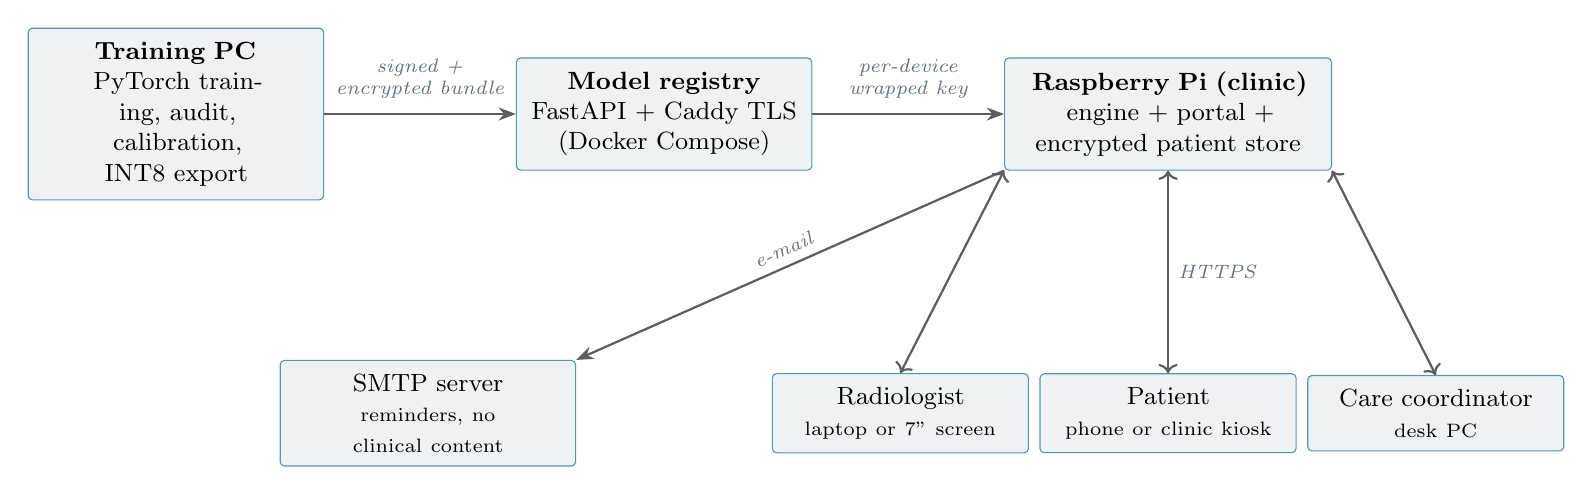
\begin{tikzpicture}[node distance=7mm and 9mm]
\node[box=3.4cm] (pc) at (0,0) {\textbf{Training PC}\\ PyTorch training, audit,\\ calibration, INT8 export};
\node[box=3.4cm] (reg) at (6.2,0) {\textbf{Model registry}\\ FastAPI + Caddy TLS\\ (Docker Compose)};
\node[box=3.8cm] (pi) at (12.6,0) {\textbf{Raspberry Pi (clinic)}\\ engine + portal +\\ encrypted patient store};
\node[box=2.9cm] (doc) at (9.2,-3.8) {Radiologist\\ \scriptsize laptop or 7" screen};
\node[box=2.9cm] (pat) at (12.6,-3.8) {Patient\\ \scriptsize phone or clinic kiosk};
\node[box=2.9cm] (coord) at (16,-3.8) {Care coordinator\\ \scriptsize desk PC};
\node[box=3.4cm] (mail) at (3.2,-3.8) {SMTP server\\ \scriptsize reminders, no clinical content};
\draw[arr] (pc) -- node[lab, above=2pt]{signed +\\ encrypted bundle} (reg);
\draw[arr] (reg) -- node[lab, above=2pt]{per-device\\ wrapped key} (pi);
\draw[arr, <->] (pi.south) -- node[lab, right]{HTTPS} (pat.north);
\draw[arr, <->] (pi.south west) -- (doc.north);
\draw[arr, <->] (pi.south east) -- (coord.north);
\draw[arr] (pi.south west) -- node[lab, above, sloped]{e-mail} (mail.north east);
\end{tikzpicture}}
\caption{Components. The model leaves the training PC only as a signed, encrypted bundle. Patient data never leaves the
clinic device; outgoing e-mails carry no clinical content.}
\end{figure}

\subsection{Technology stack}
\begin{table}[H]\centering\small
\begin{tabularx}{\linewidth}{@{}lX@{}}
\toprule
\textbf{Layer} & \textbf{Technology and role} \\
\midrule
Model training & PyTorch, timm (ResNet-50, ImageNet init), AMP bf16, EMA weights, AdamW, cosine schedule \\
Data handling & NumPy, OpenCV, pydicom, nibabel (NIfTI), SciPy; flip-aware NCC deduplication; pandas manifests \\
Evaluation & scikit-learn metrics, bootstrap confidence intervals, McNemar tests, CAM faithfulness (pointing, ROAD) \\
Export and inference & ONNX, ONNX Runtime with static INT8 quantisation (QDQ), CPU only, no PyTorch on the device \\
Uncertainty & temperature scaling, class-conditional conformal prediction, multi-layer Mahalanobis OOD \\
Model security & OpenSSF Model Signing (ECDSA P-256), AES-256-GCM, X25519 + HKDF-SHA256 key wrapping \\
Registry & FastAPI, SQLite (named Docker volume), Caddy (TLS, local CA), Docker Compose \\
Clinic portal & Flask, Jinja2, gunicorn, SQLite (WAL), server-rendered HTML + one self-hosted JS file \\
Patient data security & AES-256-GCM blob store, Argon2id passwords, TOTP two-step sign-in, CSRF tokens, strict CSP, hash-chained audit log \\
Device & Raspberry Pi 5 (8\,GB) and Pi 4 (4\,GB), Raspberry Pi OS (Debian 13), Caddy HTTPS, nftables firewall, systemd units, Tailscale Funnel for remote access \\
Kiosk & labwc (Wayland), Chromium in kiosk mode, locked-down user, built-in touch keyboard \\
Interface & IBM Plex Sans and Plex Mono (self-hosted), token-based design system, canvas 3D brain renderer \\
Testing & pytest (164 automated tests), live end-to-end registry check, scripted browser walk-through (this report's figures) \\
\bottomrule
\end{tabularx}
\caption{Technology stack.}
\end{table}

% ================================================================================================ 4
\section{Data and leakage control}
\subsection{Two-dimensional training data}
Training uses BRISC 2025, figshare (Cheng 2015) and the Nickparvar collection; BDNeuro-MRI is an external test set.
Every image is compared with every other using a flip-aware normalised cross-correlation of $64\times64$ thumbnails.
A copy threshold of 0.98 sits in an empty gap of the similarity distribution; a same-patient threshold of 0.94 was
calibrated on figshare's true patient identifiers ($\le$1\% false links). Splits are grouped so that copies and
same-patient images never straddle train and test.

\begin{table}[H]\centering\small
\begin{tabular}{@{}lr@{}}
\toprule
\textbf{Finding} & \textbf{Count} \\
\midrule
BRISC official test images that are copies of training images & 566 / 1{,}000 (462 mirrored) \\
Nickparvar images byte-identical to BRISC & 4{,}775 / 7{,}200 \\
figshare images that are near-duplicates of BRISC & 2{,}873 / 3{,}064 \\
BDNeuro images that are copies or mirrors of BRISC & 3{,}768 / 5{,}941 \\
\bottomrule
\end{tabular}
\caption{Leakage found in public brain-tumour MRI collections.}
\end{table}

\subsection{Three-dimensional patient studies}
After the radiologist's feedback the system was evaluated on complete studies. Only the T1 post-contrast volume and the
tumour mask are kept per patient.
\begin{table}[H]\centering\small
\begin{tabularx}{\linewidth}{@{}llrX@{}}
\toprule
\textbf{Dataset} & \textbf{Class} & \textbf{Patients} & \textbf{Role and licence} \\
\midrule
BraTS 2023 adult glioma & glioma & 300 & development; research use (Synapse) \\
BraTS 2023 meningioma & meningioma & 300 & development; CC BY-NC \\
NHNN pituitary MRI & pituitary & 60 & development, held-out part tested; CC BY \\
IXI healthy volunteers & no tumour & 581 & 30\% calibration, 70\% test, never trained on; CC BY-SA 3.0 \\
BraTS-Africa & glioma & 146 & external test (pending); CC BY 4.0 \\
\bottomrule
\end{tabularx}
\caption{3D datasets. Splits are by patient; a cross-dataset similarity check excluded 29 IXI volunteers whose
images were already in the 2D training data.}
\end{table}
Large archives were not downloaded whole: the pituitary set (47\,GB) and BraTS were read with HTTP range requests, so
only the needed files (about 1.2\,GB for 600 BraTS patients) were transferred.

% ================================================================================================ 5
\section{Model}\label{sec:model}
\subsection{Architecture}
A ResNet-50 backbone at output stride 8 produces a $28\times28$ feature map $A$. An FPN segmentation head predicts the
lesion probability $p$. The classifier uses \emph{lesion-attention pooling}:
\begin{equation}
z_c = b_c + \sum_{ij} a_{ij}\, W_c^{\top} A_{ij}, \qquad a_{ij} = \frac{p_{ij} + \varepsilon}{\sum_{kl} (p_{kl} + \varepsilon)},
\end{equation}
where $p$ is the detached segmentation probability pooled to the feature grid and $\varepsilon = 0.005$. With no lesion
the weights are uniform (ordinary average pooling). The exact class-evidence map $S_c(ij) = a_{ij} W_c^{\top} A_{ij}$
sums to the logit (HiResCAM form), so the Grad-CAM shown to the radiologist is an exact decomposition of the decision,
not an approximation, and it is lesion-focused by construction.

\subsection{Two-dimensional results (v1, deployed INT8 graph)}
\begin{table}[H]\centering\small
\begin{tabular}{@{}lccc@{}}
\toprule
\textbf{Metric} & \textbf{v0} & \textbf{v1 (deployed)} & \textbf{v1, 3 seeds} \\
\midrule
Test macro-F1 [95\% CI] & 0.935 & \textbf{0.944} [0.926, 0.959] & 0.938 $\pm$ 0.007 \\
External BDNeuro macro-F1 & 0.729 & \textbf{0.836} & 0.827 $\pm$ 0.012 \\
Grad-CAM evidence inside tumour & 0.150 & \textbf{0.728} (98\% of ceiling) & 0.713 $\pm$ 0.018 \\
Pointing game & 0.525 & \textbf{0.992} & 0.981 $\pm$ 0.019 \\
95\% prediction-set coverage & 0.867 & \textbf{0.911} (target 0.93) & 0.917 $\pm$ 0.006 \\
\bottomrule
\end{tabular}
\caption{Single-image results on the leakage-free test set (799 images).}
\end{table}

\subsection{Whole-study evaluation and model v2}
For a study, 36 slices are taken in three planes (12 axial, 12 coronal, 12 sagittal), each is analysed, and the patient
result is the mean of the five slices most suggestive of tumour (\emph{top-k}, chosen on calibration patients only).
Targets were fixed before testing.
\begin{table}[H]\centering\small
\begin{tabular}{@{}lccc@{}}
\toprule
\textbf{Held-out patients} & \textbf{Target} & \textbf{v1} & \textbf{v2 (\texttt{mri/0.3.0})} \\
\midrule
Tumour-type macro-F1 (159 patients) & $\ge 0.85$ & 0.71 & \textbf{0.98} \\
Slice tumour AUROC (5{,}724 slices) & $\ge 0.90$ & 0.72 & \textbf{0.95} \\
Healthy false-alarm rate (IXI, 380) & $\le 10\%$ & 23\% & \textbf{5\%} \\
\midrule
Glioma accuracy (76) & & 54\% & 100\% \\
Meningioma accuracy (68) & & 87\% & 91\% \\
Pituitary accuracy (15) & & 53\% & 100\% \\
Healthy volunteers correct (380) & & 77\% & 95\% \\
\bottomrule
\end{tabular}
\caption{Patient-level results. v2 keeps v1's architecture and preprocessing and adds slices from 3D training patients
(tumour and tumour-free slices of the same scans).}
\end{table}
The test patients come from the same datasets as the training patients; the external whole-study test (BraTS-Africa)
and two further training seeds remain to be done.

% ================================================================================================ 6
\section{Explainability and uncertainty}
\begin{itemize}
\item \textbf{Grad-CAM (exact).} Shown on the key slices with the lesion outline from the segmentation head. The
INT8 decomposition error is about $10^{-7}$.
\item \textbf{Calibration.} Temperature scaling fitted on a dedicated calibration split of the deployed INT8 graph
(expected calibration error 0.049 to 0.030 on test).
\item \textbf{95\% prediction set.} Class-conditional conformal prediction; a set with more than one class marks the
study for expert review.
\item \textbf{Out-of-distribution detection.} A multi-layer Mahalanobis score with a warning threshold (95\% of
validation) and a reject threshold (99.5\%). Rejected inputs show no diagnosis.
\item \textbf{Review flags.} Thresholds calibrated on validation data, for example the share of Grad-CAM evidence
inside the predicted lesion.
\end{itemize}
A local 1.7B language model was evaluated as a report assistant. About 4\% of its verified answers still contained a
clear error, mostly misreading statistics, so it was removed from the portal and remains only as a research
experiment.

% ================================================================================================ 7
\section{Edge optimisation and deployment}
The device runs no PyTorch: preprocessing is shared code (NumPy and OpenCV) with a fingerprint check against the
bundle, and inference is ONNX Runtime on the CPU.
\begin{table}[H]\centering\small
\begin{tabular}{@{}lcc@{}}
\toprule
\textbf{Measure} & \textbf{Raspberry Pi 5} & \textbf{PC (i7)} \\
\midrule
Single image, full analysis (median / p95) & 238 / 250\,ms & 97\,ms \\
Whole study (36 slices + key-slice overlays) & 8--14\,s & 3--6\,s \\
Peak memory, large 0.5\,mm study & 2.5\,GB & -- \\
Pi vs PC agreement (40 scans) & 40/40, CAM $r \ge 0.997$ & -- \\
Model size (INT8) & \multicolumn{2}{c}{24.7\,MB (FP32 96.6\,MB)} \\
\bottomrule
\end{tabular}
\caption{Latency and parity. Only one whole-study analysis runs at a time to bound memory.}
\end{table}
The installer (\texttt{edge/install\_pi.sh}) is idempotent and sets up the Python environment with pinned versions,
Caddy HTTPS, the firewall, the portal key and database, systemd services, model sync, and optionally the kiosk.

% ================================================================================================ 8
\section{Model security and storage}
\begin{figure}[H]\centering
\resizebox{\linewidth}{!}{%
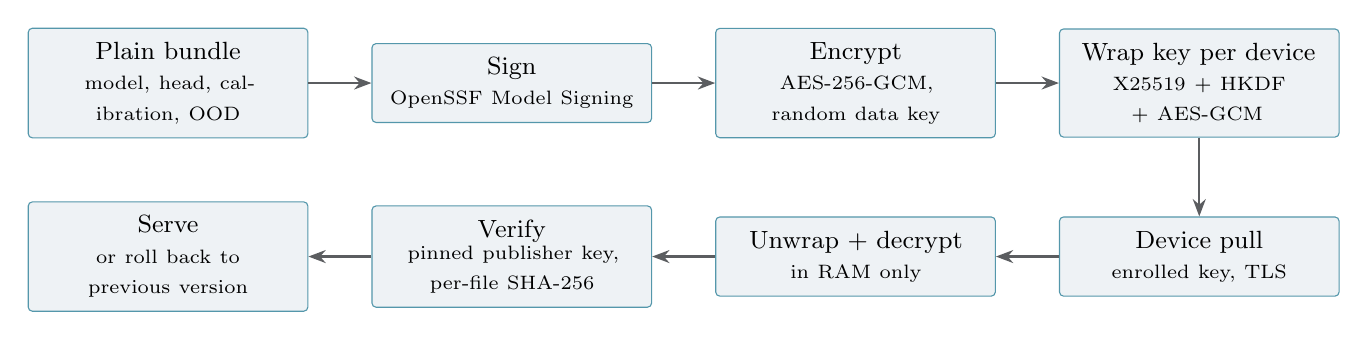
\begin{tikzpicture}[node distance=6mm and 8mm]
\node[box=3.2cm] (b) {Plain bundle\\ \scriptsize model, head, calibration, OOD};
\node[box=3.2cm, right=of b] (s) {Sign\\ \scriptsize OpenSSF Model Signing};
\node[box=3.2cm, right=of s] (e) {Encrypt\\ \scriptsize AES-256-GCM, random data key};
\node[box=3.2cm, right=of e] (w) {Wrap key per device\\ \scriptsize X25519 + HKDF + AES-GCM};
\node[box=3.2cm, below=10mm of w] (d) {Device pull\\ \scriptsize enrolled key, TLS};
\node[box=3.2cm, left=of d] (u) {Unwrap + decrypt\\ \scriptsize in RAM only};
\node[box=3.2cm, left=of u] (v) {Verify\\ \scriptsize pinned publisher key,\\ per-file SHA-256};
\node[box=3.2cm, left=of v] (r) {Serve\\ \scriptsize or roll back to previous version};
\draw[arr] (b)--(s); \draw[arr] (s)--(e); \draw[arr] (e)--(w); \draw[arr] (w)--(d);
\draw[arr] (d)--(u); \draw[arr] (u)--(v); \draw[arr] (v)--(r);
\end{tikzpicture}}
\caption{Model distribution. The signing key never leaves the training PC; the server sees only public keys and
ciphertext; the device stores only ciphertext.}
\end{figure}
\begin{itemize}
\item \textbf{Provenance.} Bundles are signed with OpenSSF Model Signing. The device pins the publisher's public key at
enrolment and never fetches it from the server, so a compromised server cannot substitute a model.
\item \textbf{Confidentiality.} Envelope encryption: the bundle is encrypted once with AES-256-GCM; the data key is
wrapped separately for every enrolled device with X25519 ECDH, HKDF-SHA256 and AES-GCM. The model name and version are
bound as associated data, so a key or ciphertext cannot be replayed against another version.
\item \textbf{Enrolment and revocation.} One-time enrolment tokens; per-device API keys; revoked devices receive 403.
\item \textbf{Storage on the device.} Only the encrypted blob and its manifest are stored
(\texttt{/var/lib/neuroedge/models}); the stored blob measures 8.000 bits per byte of entropy. Decryption happens in
memory at start-up, and if the newest version fails verification the previous one is used.
\item \textbf{Live verification.} \texttt{server/e2e\_check.py} runs 16 checks against the live registry (verified TLS,
signature and decryption, byte-identical files, ciphertext-only storage, 401 on forged keys, a single flipped
ciphertext bit detected, another device unable to decrypt, 403 after revocation). All 16 pass for \texttt{mri/0.3.0}.
\end{itemize}

% ================================================================================================ 9
\section{Portal security and patient-data storage}
\begin{table}[H]\centering\small
\begin{tabularx}{\linewidth}{@{}lX@{}}
\toprule
\textbf{Concern} & \textbf{Implementation} \\
\midrule
Transport & HTTPS through Caddy with a local certificate authority; the Flask app listens on loopback only; nftables admits only SSH, HTTP(S) and mDNS \\
Scans, overlays, reports & Encrypted blob store: AES-256-GCM, a 12-byte nonce per file, the case and file kind as associated data so files cannot be swapped between cases; key in \texttt{/etc/neuroedge/portal.key} (root and service only) \\
Records & SQLite in WAL mode; the database stores SHA-256 hashes of every scan and signed report snapshot \\
Accounts & Argon2id password hashing, account lock-out, optional mandatory two-step sign-in (TOTP with recovery codes) for staff \\
Sessions and forms & HttpOnly, SameSite=Strict, \texttt{\_\_Host-} cookies; CSRF token on every form; idle and absolute session timeouts \\
Browser hardening & Content Security Policy allows only same-origin scripts and styles, no inline code; frame and referrer protection \\
Access control & Roles (patient, radiologist, coordinator) and object-level checks; patients never receive AI overlays or probabilities \\
Accountability & Hash-chained, tamper-evident audit log of every view, signature and change, verifiable from the command line \\
Privacy & Consent records, full data export for the patient, deletion requests, e-mails with no clinical content \\
\bottomrule
\end{tabularx}
\caption{Security controls in the clinic portal.}
\end{table}

% ================================================================================================ 10
\section{The clinical workflow, step by step}
The figures in this section were produced by a scripted walk-through of the running system
(\texttt{docs/report/capture.py}): a fresh demo database, a real whole-study MRI upload analysed by model v2, and the
e-mails exactly as the portal generated them.

\subsection{Device home and sign-in}
\shot{01_device_home}{Device home. The portal's front page: a rotating brain surface reconstructed from a real MRI
study, a status bar (network address, storage, clock) and the two entry points. No patient data appears here.}
\shot[0.42]{01b_device_home_7inch}{The same page on the official 7-inch touch display (800$\times$480).}
\shot{02_login}{Sign-in, with separate patient and clinician tabs.}

\subsection{Patient: registration and upload}
\shot{03_register}{Patient registration with explicit consent for storage and review.}
\shot{04_patient_dashboard_new}{A new patient's dashboard.}
\shot{05_patient_upload}{Uploading a whole MRI study (a NIfTI volume) with a note for the radiologist. Single images,
ZIP archives and multi-file DICOM series are also accepted.}
\shot{06_patient_case_received}{After upload: the study is received and the progress tracker shows that it is waiting
for the radiologist. The patient sees no AI result.}

\subsection{Radiologist: worklist, review and signature}
\shot{07_doctor_worklist}{The reading worklist, prioritised by the AI's review flags, with waiting times and status.}
\shot{08_doctor_case_review}{Case review. The viewer shows Grad-CAM on key slice 1; the slice strip below shows the tumour
likelihood of all 36 slices (key slices in amber). The findings panel gives the study-level probabilities, the 95\%
prediction set and the lesion measurements.}
\shot{09_doctor_case_combined}{Combined view: Grad-CAM with the lesion outline from the segmentation head.}
\shot{10_doctor_case_other_slice}{Scrolling through the study: a non-key slice is shown without overlays, as the
radiologist reads the whole series.}
\shot{11_doctor_sign_report}{Signing the report. The radiologist states agreement with the AI, writes findings and a
recommendation, and chooses the follow-up step (here a consultation within two weeks). The signature requires the
password again.}
\shot{12_doctor_signed}{The signed report is released to the patient and the follow-up plan is created.}
\shot{13_doctor_availability}{Consultation hours and days off, which define the slots patients can book.}

\subsection{Patient: report, next step and booking}
\shot{14_patient_dashboard_next_step}{The patient's dashboard after signing: the care-progress tracker and the next
step requested by the radiologist.}
\shot{15_patient_report}{The signed radiology report, as the patient sees it (printable). It contains the
radiologist's diagnosis and findings only, never AI output.}
\shot{16_patient_booking}{Booking a consultation from the radiologist's free slots.}
\shot{17_patient_booked}{Booking confirmation with a calendar invitation.}
\shot{18_patient_appointments}{The patient's appointments, with options to reschedule or cancel.}

\subsection{E-mails sent along the way}
E-mails are sent through the clinic's SMTP server (here saved as files in demo mode). They carry no diagnosis or other
medical details; the patient signs in to read the report.
\begin{figure}[H]\centering
\begin{subfigure}{0.49\linewidth}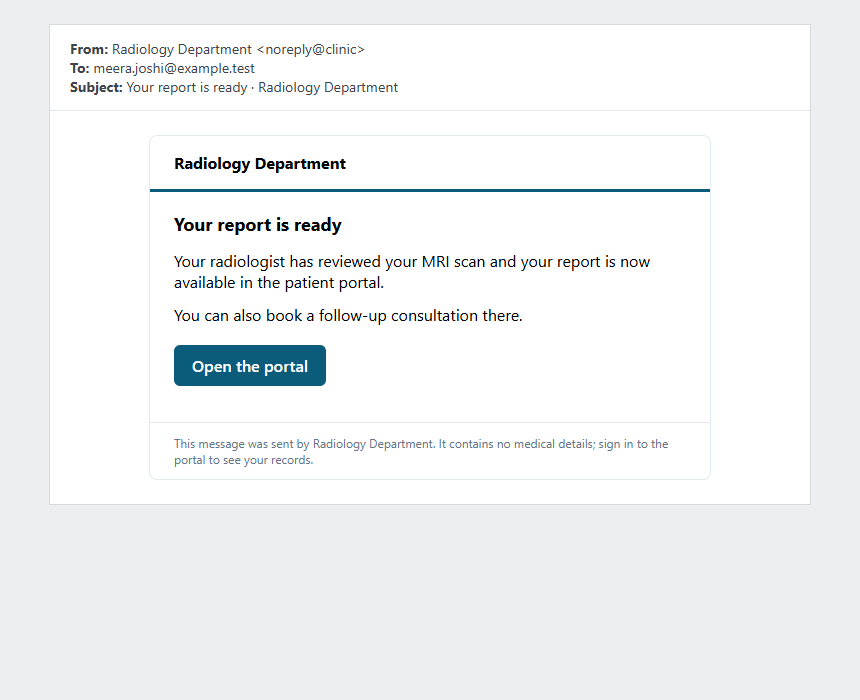
\includegraphics[width=\linewidth]{40_email_1}\caption{Report ready.}\end{subfigure}\hfill
\begin{subfigure}{0.49\linewidth}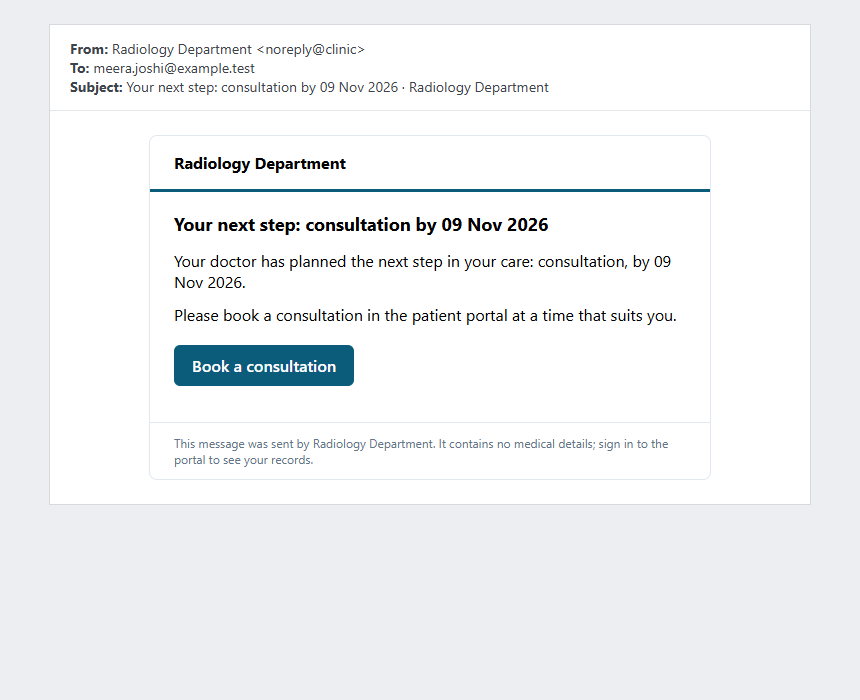
\includegraphics[width=\linewidth]{40_email_2}\caption{Next step requested.}\end{subfigure}
\\[6pt]
\begin{subfigure}{0.49\linewidth}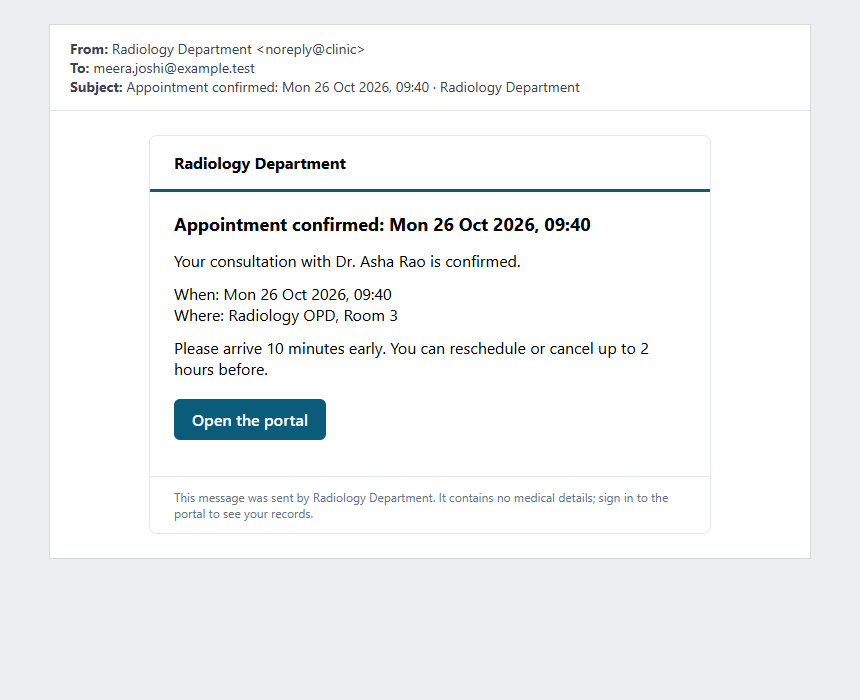
\includegraphics[width=\linewidth]{40_email_3}\caption{Appointment confirmed.}\end{subfigure}
\caption{The three e-mails generated in this walk-through.}
\end{figure}

\subsection{Radiologist: schedule and analytics}
\shot{19_doctor_schedule}{The radiologist's consultation schedule with the patient's booking.}
\shot[0.92]{20_analytics}{Analytics. The care-loop section (closure and loss-to-follow-up rates, a funnel from signed
report to closed loop, risk bands with their reasons, distance to care, districts, next steps, referrals, outreach and
consultations), followed by reading performance and AI agreement with the signed diagnosis. Every rate shows its
denominator.}

\subsection{Care coordinator: follow-up and administration}
\shot{21_followup_worklist}{The follow-up worklist, ranked by an explainable risk score (days overdue, missed visits,
unanswered calls, contact details, open referral, distance). The score never uses the diagnosis or any AI output.}
\shot{22_patient_record}{A patient record with the unified timeline, contact log, follow-up plan and referrals.}
\shot{23_walkin_registration}{Walk-in registration at the desk, with a first scan; no e-mail address is needed.}
\shot{24_referrals}{Referral tracking from signed letter to closed.}
\shot{25_admin_users}{User management.}
\shot{26_audit_log}{The tamper-evident audit log, verified on every view.}
\shot{27_admin_system}{System status: model version and signature check, storage, security, audit chain.}
\shot{28_email_outbox}{The e-mail outbox with delivery status and retries.}
\shot{29_admin_settings}{Department settings, including reminder and escalation timings.}

\subsection{The device's own screen}
\begin{figure}[H]\centering
\begin{subfigure}{0.49\linewidth}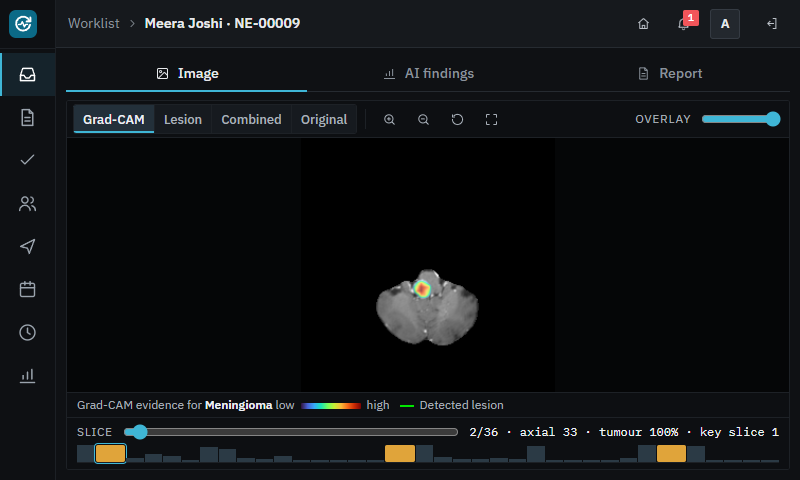
\includegraphics[width=\linewidth]{30_kiosk_case_review}\caption{Case review as tabs.}\end{subfigure}\hfill
\begin{subfigure}{0.49\linewidth}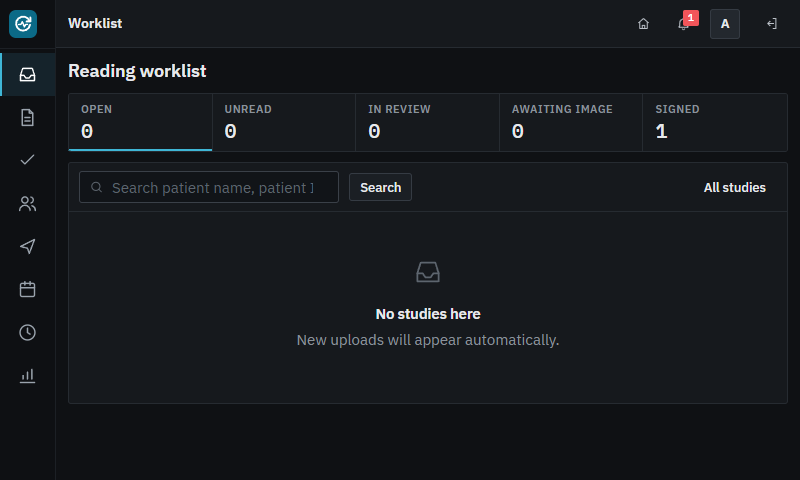
\includegraphics[width=\linewidth]{31_kiosk_worklist}\caption{Worklist.}\end{subfigure}
\\[6pt]
\begin{subfigure}{0.49\linewidth}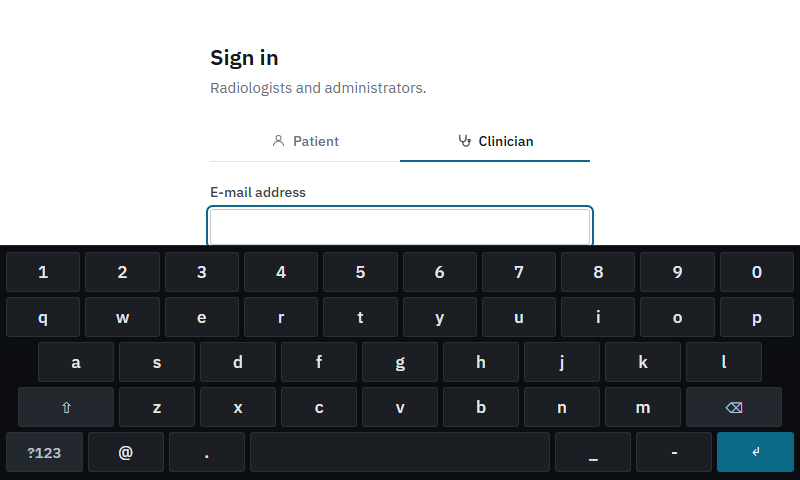
\includegraphics[width=\linewidth]{32_kiosk_keyboard}\caption{Built-in touch keyboard.}\end{subfigure}
\caption{Kiosk mode on the 7-inch display (800$\times$480). The case page becomes Image / AI findings / Report tabs with
the image filling the screen; touch targets are at least 44\,px.}
\end{figure}

% ================================================================================================ 11
\section{Device deployment}
\begin{itemize}
\item \textbf{Raspberry Pi 5 (8\,GB).} The main clinic device: portal, model \texttt{mri/0.3.0}, remote access through
Tailscale Funnel.
\item \textbf{Raspberry Pi 4 (4\,GB) with the official 7-inch display.} Installed from a newly written SD card
(Raspberry Pi OS, first-boot configuration with key-only SSH), enrolled with the registry, model verified, kiosk
running on the screen. The language model is not installed, which keeps memory free for whole-study analysis.
\item \textbf{Kiosk.} A locked-down \texttt{kiosk} user without password, sudo or SSH logs in on the display and opens the
device home in Chromium. Keyboard shortcuts that could leave the kiosk are disabled, and the screen returns to the
device home after three idle minutes.
\end{itemize}
Problems found only on real hardware were fixed in the installer, for example SNI-less TLS by IP address,
first-boot-only network configuration, the operating system's desktop auto-login overriding the kiosk, and a
certificate tool waiting for a password prompt.

% ================================================================================================ 12
\section{Testing and verification}
\begin{itemize}
\item \textbf{163 automated tests} (pytest): CAM exactness, cryptography and tamper detection, leakage deduplication,
portal roles and object-level access, CSRF and lock-out, the encrypted store, audit-chain verification, appointments,
reminders, follow-up plans and risk score, whole-series upload and its safety checks (mixed patients or series
refused), analytics figures on a seeded clinic, and the device page (no patient data).
\item \textbf{Registry end-to-end check}: 16/16 against the live server.
\item \textbf{Pi--PC parity}: 40/40 identical predictions.
\item \textbf{Browser verification} at 800$\times$480, 1280$\times$720 and desktop sizes, with no Content Security
Policy violations; the walk-through in Section~10 is itself an end-to-end test of the main workflow.
\end{itemize}

% ================================================================================================ 13
\section{Limitations and future work}
\begin{itemize}
\item Model v2 is one training seed; whole-study results are on held-out patients of the training datasets. The
external BraTS-Africa test and two more seeds are pending.
\item The healthy-volunteer set (IXI) is non-contrast T1; the 95\% set is calibrated on slices, not on patients.
\item Single-image prediction-set coverage is 0.91 against a 0.93 target; calibration per data source is planned.
\item Measured Pi 4 whole-study latency is still to be recorded.
\item BraTS data is licensed for research and non-commercial use.
\item Planned: SMS and WhatsApp reminders in local languages, a PACS connection, and a pilot at a health centre.
\end{itemize}

\end{document}
